%LaTeX-2e-File, Liedtke, 20140724.
%Inhalt: Einf"uhrung der Ableitung.
%zuletzt bearbeitet: 20140922.

%\begin{MContent}

%\begin{MXContent}{Zur Idee der Ableitung als Ma"s f"ur die "Anderungsrate der Funktionswerte}{Zur Idee der Ableitung}{STD}
\begin{MXContent}{Relative �nderungsrate einer Funktion}{Relative �nderungsrate}{STD}

Untersuchen wir eine Funktion $f: [a, b] \rightarrow \R$ und skizzieren diese in einen Graphen (siehe unten). Unser Ziel ist die Beschreibung der �nderungsrate dieser Funktion an einer beliebigen Stelle $x_0$ zwischen $a$ und $b$. Die �nderungsrate k�nnen wir �ber die Ableitung der Funktion bestimmen. Dazu wollen wir m�glichst einfache Rechenregeln verwenden.

%----------------------------------------------------------------------------------------
%Bild:
\begin{center}
\ifttm
\MGraphicsSolo{\MPfadBilder/jb07A1_Funktionsgraph.png}{scale=0.5}
\else
%Datei: {\MPfadBilder/jb07A1_Funktionsgraph.tex}
\begin{small}
\renewcommand{\jTikZScale}{0.7}
\tikzsetnextfilename{jb07A1_Funktionsgraph}
\begin{tikzpicture}[line width=1.5pt,scale=\jTikZScale, %
declare function={
  x0 = 2;
  x1 = 4;
  fkt(\x) = 1/4 * (\x - 1)*(\x - 1) + 0.75;
  rT = 1.6; % relative Translation der Beschriftung $\Delta(f)$
%  Tangente(\x) = 1/2 * (\x - 2) + 1;
}
] %[every node/.style={fill=white}] 
%Koordinatenachsen:
\draw[->] (-0.6, 0) -- ({x1+1}, 0) node[below left]{$x$}; %x-Achse
\draw[->] (0, -0.6) -- (0, {fkt(x1)+1}) node[below left]{$y$}; %y-Achse
%Achsenbeschriftung:
\foreach \x in {1, 2, 3, 4} \draw (\x, 0) -- ++(0, -0.1); %
% node[below] {$\x$}; 
\foreach \y in {1, 2, 3} \draw (0, \y) -- ++(-0.1, 0); %
% node[left] {$\y$};
%\node[below left] at (0, 0) {$0$};
%Hilfslinien:
\draw[color=black!50!white,style=dashed] (x1, {fkt(x0)}) -- (x1, {fkt(x1)});
\draw[color=black!50!white,style=dotted] (x0, {fkt(x0)}) -- (x1, {fkt(x0)});
%Funktion:
\draw[domain=0.5:x1,samples=120,color=\jccolorfkt] %
 plot (\x, {fkt(\x)});
%Punkte und Hilfslinien:
\filldraw[color=black,fill=black] (x0, 0) circle (1pt);
\node[below] at (x0, -0.1) {$x_0$};
\filldraw[color=black,fill=black] (x0, {fkt(x0)}) circle (1pt);
%
\filldraw[color=black,fill=black] (x1, 0) circle (1pt);
\node[below] at (x1, -0.1) {$x$};
%
\filldraw[color=black,fill=black] (x1, {fkt(x0)}) circle (1pt);
\filldraw[color=black,fill=black] (x1, {fkt(x1)}) circle (1pt);
%Beschriftung:
\draw[line width=0.8pt, rounded corners=4pt] %
 ({x1 + rT + 0.0}, 1.0) -- ({x1 + rT + 0.2}, 1.0) -- ({x1 + rT + 0.2}, 2.0) %
 -- ({x1 + rT + 0.4}, 2.0);
\draw[line width=0.8pt, rounded corners=4pt] %
 ({x1 + rT + 0.4}, 2.0) %
 -- ({x1 + rT + 0.2}, 2.0) -- ({x1 + rT + 0.2}, 3.0) -- ({x1 + rT + 0.0}, 3.0);
%
\node[right] at ({x1+rT+0.5}, 2) {$\Delta(f) = f(x) - f(x_0)$};
%
\node[left] at (-0.5, {fkt(x0)}) {$f(x_0)$};
\node[left] at (-0.5, {fkt(x1)}) {$f(x)$};
\end{tikzpicture}
\end{small}
\fi
\end{center}
%Bildende.
%----------------------------------------------------------------------------------------

Halten wir $x_0$ und den entsprechenden Funktionswert $f\left(x_0\right)$ fest und w�hlen eine weitere beliebige, aber variable Stelle $x$ zwischen $a$ und $b$, sowie ihren Funktionswert $f\left(x\right)$ aus.  Verbinden wir die beiden Punkte, die wir so gefunden haben, auf dem k�rzesten Weg miteinander, so erhalten wir eine Gerade, die wir mithilfe einer Geradengleichung beschreiben k�nnen. Als Steigung dieser Geraden erhalten wir den Differenzenquotienten

\[
\frac{\Delta(f)}{\Delta(x)} = \frac{f(x) - f(x_0)}{x - x_0},
\]

der beschreibt, wie sich die Funktionswerte von $f$ \textbf{im Mittel} zwischen $x_0$ und $x$ �ndern. Wir haben also eine \textbf{mittelere �nderungsrate} der Funktion $f$ im Intervall $[x_0, x]$ gefunden. Dieser Quotient wird auch als \textbf{relative �nderung} bezeichnet.

Bilden wir den Grenzwert f�r $x \rightarrow x_0$, stellen wir fest, dass die Gerade, die den Graphen der Funktion in den Punkten $\left(x_0, f\left(x_0\right)\right)$ und $\left(x, f\left(x\right)\right)$ schneidet, immer mehr zu einer Tangenten an den Graphen im Punkt $\left(x_0, f\left(x_0\right)\right)$ wird. Auf diese Weise k�nnen wir uns also der �nderungsrate der Funktion $f$ an der Stelle $x_0$ ann�hern. Existiert dieser Grenzwert, so bezeichnen wir

\[
f'(x_0) = \lim_{x \rightarrow x_0} \frac{\Delta(f)}{\Delta(x)} 
 = \lim_{x \rightarrow x_0} \frac{f(x) - f(x_0)}{x - x_0} %%
\] 

als Ableitung von $f$ in $x_0$. Die Funktion $f$ ist dann an der Stelle $x_0$ \textbf{ableitbar} bzw. \textbf{differenzierbar}.

\begin{MExample}
  F�r $f(x)=\sqrt{x}$ ist die relative �nderung an der Stelle $x_0=1$ gegeben durch
  \[
    \frac{f(x) - f(x_0)}{x - x_0} \;=\;
    \frac{\sqrt{x}-1}{x-1} \;=\; \frac{\sqrt{x}-1}{(\sqrt{x}-1)(\sqrt{x}+1)} \;=\; \frac1{\sqrt{x}+1}\: .
  \]
  Bewegt sich nun $x$ auf $x_0=1$ zu, so erhalten wir den Grenzwert
  $$
  \lim_{x \rightarrow x_0} \frac{\Delta(f)}{\Delta(x)} \;=\; \frac12\: .
  $$
  Als Ableitung w�rde man $f'(1)=\frac12$ aufschreiben.
\end{MExample}

\begin{MExercise}
  Es sei $f(x)=x^2$ und $x_0=1$. In diesem Punkt betr�gt die relative �nderung (f�r ein $x>0$)
  
  \MEquationItem{$\displaystyle \frac{f(x) - f(1)}{x - 1}$}{\MSimplifyQuestion{20}{x+1}{4}{x}{4}{1}}.\\
  \MInputHint{Rechnen Sie den Quotienten direkt aus, ohne bekannte Ableitungswerte und Regeln aus der Schule einzusetzen.}
 
  Bewegt sich $x$ auf $x_0=1$ zu, so erhalten wir die Steigung \MParsedQuestion{5}{2}{5} von $f(x)$ im Punkt $x_0=1$.

  \begin{MHint}{L�sung}
  F�r $f(x)=x^2$ ist die relative �nderung an der Stelle $x_0=1$ gegeben durch
  \[
    \frac{f(x) - f(1)}{x - 1} \;=\;
    \frac{x^2-1}{x-1} \;=\; \frac{(x-1)(x+1)}{x-1} \;=\; x+1\: .
  \]
  Bewegt sich nun $x$ auf $x_0$ zu, so erhalten wir den Grenzwert
  $$
  \lim_{x \rightarrow 1} \frac{\Delta(f)}{\Delta(x)} \;=\; 2\: .
  $$
  Das ist die Steigung der Tangente an den Graph von $f(x)$ im Punkt $x_0=1$.
  Als Ableitung w�rde man $f'(1)=2$ aufschreiben.
  \end{MHint}  
\end{MExercise}

�ber die Formel f�r die relative �nderungsrate kann man die Ableitung nur sehr m�hsam und
auch nur f�r sehr einfache Funktionen ausrechnen. Typischerweise rechnet man die Ableitung
durch Anwendung von Rechenregeln aus und durch Einsetzen bekannter Ableitungswerte f�r bestimmte
Bausteine.

\end{MXContent}


%\MSubsubsection{Ableitung}
\begin{MXContent}{Ableitung}{Ableitung}{STD}

\begin{MXInfo}{Schreibweisen der Ableitung}
In der Mathematik, sowie auch in den Natur- und Ingenieurwissenschaften werden verschiedene Schreibweisen der Ableitung �quivalent verwendet:
\[
f'(x_0) = \frac{\MD f}{\MD x}(x_0) = \frac{\MD}{\MD x}f(x_0)%%
\]
Diese Schreibweisen haben jeweils die Bedeutung der Ableitung der Funktion $f$ in $x_0$.
\end{MXInfo}

Wenn die Ableitung mithilfe des Differenzenquotienten $\frac{f(x) - f(x_0)}{x - x_0}$ berechnet werden muss,
bietet es sich oft an, den Differenzenquotienten anders aufzuschreiben. Verwenden wir die Differenz von $x$ und $x_0$ und bezeichnen wir sie als $h := x - x_0$, 

%Bild:
\begin{center}
\ifttm
\MGraphicsSolo{\MPfadBilder/jb07A1_AbstandReellerZahlen.png}{scale=0.5}
\else
%Datei: {\MPfadBilder/jb07A1_AbstandReellerZahlen.tex}
\begin{small}
\renewcommand{\jTikZScale}{0.7}
\tikzsetnextfilename{jb07A1_AbstandReellerZahlen}
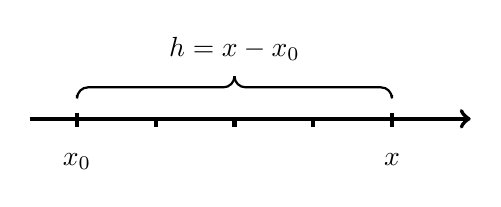
\begin{tikzpicture}[line width=1.5pt,scale=\jTikZScale, %
declare function={
  x0 = 0;
  x1 = 4;
}
] %[every node/.style={fill=white}] 
%Koordinatenachsen:
\draw[->] (-0.6, 0) -- ({x1+1}, 0); % node[below left]{$x$}; %x-Achse
%Achsenbeschriftung:
\foreach \x in {0, 1, 2, 3, 4} \draw (\x, 0.0) -- ++(0, -0.1); %
\foreach \x in {0, 4} \draw (\x, 0.0) -- ++(0, +0.08); %
% node[below] {$\x$}; 
%Beschriftung:
%\draw[line width=0.8pt, rounded corners=4pt] %
% (0, 0.3) -- (0, 0.4) -- (2, 0.4) -- (2, 0.5);
\draw[line width=0.8pt, rounded corners=4pt] %
 ({x0}, 0.3) -- ({x0}, 0.4) -- ({x1/2}, 0.4) %
 -- ({x1/2}, 0.5);
\draw[line width=0.8pt, rounded corners=4pt] %
 ({x1/2}, 0.5)
 -- ({x1/2}, 0.4) -- ({x1}, 0.4) -- ({x1}, 0.3);
%
\node[above] at ({x1/2}, 0.6) {$h = x - x_0$};
%
\node[below] at ({x0}, -0.3) {$x_0$};
\node[below] at ({x1}, -0.3) {$x$};
\end{tikzpicture}
\end{small}
\fi
\end{center}
%Bildende.

k�nnen wir den Differenzenquotienten mit $x = x_0 + h$ umschreiben:
\[
\frac{f(x) - f(x_0)}{x - x_0} = \frac{f(x_0 + h) - f(x_0)}{h}.
\]
Beachten Sie, dass wir keine Voraussetzung dar�ber getroffen haben, ob $x$ gr��er oder kleiner als $x_0$ ist. Die Gr��e $h$ kann daher positive oder negative Werte annehmen. Um die Ableitung der Funktion $f$ zu bestimmen, muss nun der Grenzwert f�r $h \rightarrow 0$ berechnet werden: 
\[
f'(x_0) = \lim_{x \rightarrow x_0} \frac{f(x) - f(x_0)}{x - x_0} %
 = \lim_{h \rightarrow 0} \frac{f(x_0 + h) - f(x_0)}{h}
\]
Wenn dieser Grenzwert existiert, ist eine Funktion differenzierbar. Viele der h�ufig benutzten Funktionen sind differenzierbar. Ein einfaches Beispiel daf�r, dass eine Funktion nicht unbedingt differenzierbar ist, ist die Betragsfunktion $f(x) := |x|$.

\begin{MExample}
Die Betragsfunktion (siehe Modul \MRef{VBKM06}, Abschnitt \MRef{VBKM06_sec:betrag}) ist an der Stelle $x_0 = 0$ nicht differenzierbar.
Sehen wir uns den Differenzenquotienten f�r $f$ an der Stelle $x_0 = 0$ an:
\[
\frac{f(0+h) - f(0)}{h} = \frac{|h| - |0|}{h} = \frac{|h|}{h}
\]
Da $h$ gr��er oder kleiner als $0$ sein kann, m�ssen wir beide F�lle unterscheiden. Beginnen wir mit $h > 0$. Dann ist $\frac{|h|}{h} = \frac{h}{h} = 1$. Untersuchen wir den Fall $h < 0$, so finden wir, dass $\frac{|h|}{h} = \frac{-h}{h} = -1$ ist. Der Grenzwert des Differenzenquotienten h�ngt also von Wahl von $h$ ab und ist damit nicht eindeutig bestimmt. Der Grenzwert des Differenzenquotienten an der Stelle $x_0 = 0$ existiert nicht. Daher ist die Betragsfunktion an der Stelle $x_0 = 0$ nicht differenzierbar.

Der Verlauf des Graphen "andert seine Richtung an der Stelle $(0, 0)$ sprunghaft: Salopp ausgedr"uckt, weist der Funktionsgraph an der Stelle $(0, 0)$ einen Knick auf.
%Bild:
\begin{center}
\ifttm
\MUGraphicsSolo{\MPfadBilder/jb07A1_BspBetragsfunktion.png}{scale=0.5}{}
\else
%Datei: {\MPfadBilder/jb07A1_BspBetragsfunktion.tex}
\renewcommand{\jTikZScale}{1.0}
\tikzsetnextfilename{jb07A1_BspBetragsfunktion}
\begin{tikzpicture}[line width=1.5pt,scale=\jTikZScale]
%LaTeX-File, Liedtke, 20140916.
%VBKM-Modul 7 Differentialrechnung: Bild zur Betragsfunktion
%Bildname: jb07A2_BspBetragsfunktion
%Erstellt: 20140916, Liedtke.

%\begin{small}
%\begin{tikzpicture}[line width=1.5pt,scale=\jTikZScale, %
%declare function={
%  fkt(\x) = sin(\x r);
%}
%] %[every node/.style={fill=white}] 
%Koordinatenachsen:
\draw[->] (-3.6, 0) -- (4, 0) node[below left]{$x$}; %x-Achse
\draw[->] (0, -0.6) -- (0, 4.6) node[below left]{$y$}; %y-Achse
%Achsenbeschriftung:
\foreach \x in {-3, -2, -1, 1, 2, 3} \draw (\x, 0) -- ++(0, -0.1) %
 node[below] {$\x$};
\foreach \y in {1, 2, 3, 4} \draw (0, \y) -- ++(-0.1, 0) node[left] {$\y$};
%\node[below left] at (0, 0) {$0$};
%Funktion:
\draw[domain=-3.2:3.2,samples=120,color=\jccolorfkt] %
 plot (\x, {abs(\x)});
%Tangenten im Nullpunkt, wenn $f$ f"ur $x \leq 0$ bzw. $x \geq 0$ betrachtet 
%wird:
\draw[samples=120,color=blue!50!black] %
 (-0.5, 0.5) -- (0.5, -0.5);
\draw[samples=120,color=blue!50!black] %
 (-0.5, -0.5) -- (0.5, 0.5);
%Punkt: Markierung der Stelle $0$:
\filldraw[color=black,fill=black] (0, 0) circle (1pt);
%end of file
\end{tikzpicture}
\fi
\end{center}
%Bildende.
\end{MExample}

Auch wenn eine Funktion eine Sprungstelle hat, gibt es keine eindeutige Tangente an den Graphen und somit keine Ableitung.

%Bild:
%\ifttm
%\MUGraphics{\MPfadBilder/jb07A1_BspUnstetigeFkt.png}{scale=0.5}%
%{Funktion mit Sprungstelle in $x_0 = 1$}{}
%\else
%\begin{center}
%Datei: {\MPfadBilder/jb07A1_BspUnstetigeFkt.tex}
%\renewcommand{\jTikZScale}{1.0}
%\tikzsetnextfilename{jb07A1_BspUnstetigeFkt}
%\begin{tikzpicture}[line width=1.5pt,scale=\jTikZScale]
%LaTeX-File, Liedtke, 20140916.
%VBKM-Modul 7 Differentialrechnung: Bild einer unstetigen Funktion
%Bildname: jb07A2_BspUnstetigeFkt.
%Erstellt: 20140916, Liedtke.
%declare function={
%  fkt(\x) = (\x+1)*(\x+1)/4 + 0.5};
%}
%] %[every node/.style={fill=white}] 
%Koordinatenachsen:
%\draw[->] (-3.6, 0) -- (4, 0) node[below left]{$x$}; %x-Achse
%\draw[->] (0, -0.6) -- (0, 4.2) node[below left]{$y$}; %y-Achse
%Achsenbeschriftung:
%\foreach \x in {-3, -2, -1, 1, 2, 3} \draw (\x, 0) -- ++(0, -0.1) %
% node[below] {$\x$};
%\foreach \y in {2, 3} \draw (0, \y) -- ++(-0.1, 0) node[left] {$\y$};
%\node[below left] at (0, 0) {$0$};
%Funktion:
%\draw[domain=-2.0:1.0,samples=120,color=\jccolorfkt] %
% plot (\x, {(\x+1)*(\x+1)/4 + 0.5});
%\draw[domain=1.05:2.0,samples=120,color=\jccolorfkt] %
% plot (\x, {(\x+1)*(\x+1)/4 + 1.5});
%Tangenten in $x_0 = 1$, wenn die stetige Fortsetzung von $f$ f"ur $x \leq 1$ 
%bzw. $x \geq 1$ betrachtet wird:
%\draw[samples=120,color=blue!50!black] %
% (0.5, 1.0) -- (1.5, 2.0);
%\draw[samples=120,color=blue!50!black] %
% (0.5, 2.0) -- (1.5, 3.0);
%Punkt: Markierung der Stelle $x_0 = 1$:
%\filldraw[color=black,fill=black] (1, 0) circle (1pt);
%\end{tikzpicture}
%\end{center}
%\fi
%Bildende.

\end{MXContent}

%\end{MContent}

%end of file.

